%%%%%%%%%%%%%%%%%%%%%%% file template.tex %%%%%%%%%%%%%%%%%%%%%%%%%
%
% This is a general template file for the LaTeX package SVJour3
% for Springer journals.          Springer Heidelberg 2010/09/16
%
% Copy it to a new file with a new name and use it as the basis
% for your article. Delete % signs as needed.
%
% This template includes a few options for different layouts and
% content for various journals. Please consult a previous issue of
% your journal as needed.
%
%%%%%%%%%%%%%%%%%%%%%%%%%%%%%%%%%%%%%%%%%%%%%%%%%%%%%%%%%%%%%%%%%%%
\RequirePackage{fix-cm}
%
%\documentclass{svjour3}                     % onecolumn (standard format)
%\documentclass[smallcondensed]{svjour3}     % onecolumn (ditto)
%\documentclass[smallextended]{svjour3}       % onecolumn (second format)
\documentclass[twocolumn]{svjour3}          % twocolumn
%
\smartqed  % flush right qed marks, e.g. at end of proof
%
\usepackage{graphicx}
\graphicspath{{figs/}}
\usepackage{tikz}
\usetikzlibrary{shapes}
%
\usepackage{amsmath} 
\usepackage{mathptmx}      % use Times fonts if available on your TeX system
%
\usepackage{color, soul}
\usepackage{url}
\usepackage[numbers, square, comma, sort&compress]{natbib}
\usepackage{multirow}
% insert here the call for the packages your document requires
%\usepackage{latexsym}
% etc.
%
% please place your own definitions here and don't use \def but
% \newcommand{}{}
%
% Insert the name of "your journal" with
\journalname{Int J Soc Robot}
%

\newcommand{\eg}{{\textit{e.g.~}}}
\newcommand{\etal}{{\textit{et al.~}}}
\newcommand{\ie}{{\textit{i.e.~}}}

\hyphenation{com-mon-ly}

\begin{document}

\title{On the Dynamics of Anthropomorphism in Robotics
\thanks{This research was supported by the Swiss National Science Foundation through the National Centre of Competence in Research Robotics.}
}
\subtitle{}

%\titlerunning{Short form of title}        % if too long for running head

\author{Julia Fink         \and
        S\'{e}verin Lemaignan     \and
        Pierre Dillenbourg  %etc.
}

%\authorrunning{Short form of author list} % if too long for running head

\institute{J. Fink \and S. Lemaignan \and P. Dillenbourg \at
              Computer-Human Interaction in Learning and Instruction (CHILI) \\
              Ecole Polytechnique F\'{e}d\'{e}rale de Lausanne (EPFL) \\
              Rolex Learning Center, Station 20 \\
              CH-1015 Lausanne \\
              Switzerland \\
              Tel.: +41-21-693-2274\\
              Fax: +41-21-693-6070\\
              \email{julia.fink@epfl.ch}           %  \\
%             \emph{Present address:} of F. Author  %  if needed
           \and
           S. Lemaignan \at
              \email{severin.lemaignan@epfl.ch}
		   \and
           P. Dillenbourg \at
              \email{pierre.dillenbourg@epfl.ch}
}

\date{Received: date / Accepted: date}
% The correct dates will be entered by the editor


\maketitle

\begin{abstract}

	While anthropomorphism in robotics is a commonly discussed trait of human-robot interaction (HRI), it is paradoxically an overlooked research topic. This article attempts first at providing a comprehensive synthesis of the social phenomenon of \textit{attributing human characteristics to robots}. It draws on social sciences and psychology, as well as on a critical survey of existing literature in the HRI community, to ground the concept of \textit{anthropomorphism}. We further present different kinds of \textit{anthropomorphic design} of robots and outline their role in social robotics. We then propose to go beyond the traditional perception of anthropomorphism as a static feature. We suggest to understand anthropomorphism as a dynamic, context-dependent process. This also provides an account of the so-called \textit{novelty effect}. To this end, we introduce an initial function of anthropomorphism that models the phenomenon along three interaction phases. Our function is supported by results of a long-term study that we conducted in a real human environment.


%	This article synthesizes the social phenomenon of attributing human characteristics to robots, and illustrates the role of human-like form and human social behavior cues in the design of robots. We draw on backgrounds from social sciences and psychology to first provide a common ground for the understanding of  anthropomorphism. The theoretical background is featured by an overview of different kinds of anthropomorphic design in robots. We also provide a comprehensive summary and critical comparison of findings from experiments studying anthropomorphism in human-robot interaction. Finally, we propose to understand anthropomorphism as a dynamic phenomenon which is not only determined by 1) \textit{individual characteristics} of the human user, and 2) the \textit{anthropomorphic design of the robot}, but might also be impacted by 3) \textit{dynamics}, such as \textit{time} and the \textit{context of use}. Consequently, we propose different levels of anthropomorphism that might shift with increased time of interaction and the context of use of a robot.
	


\keywords{
	Anthropomorphism \and
	Design \and    
    Human-Robot Interaction \and
    Social Issues in Robotics \and
    Acceptance of Robots}
% \PACS{PACS code1 \and PACS code2 \and more}
% \subclass{MSC code1 \and MSC code2 \and more}
\end{abstract}


%%%%%%%%%%%%%%%%%%%%%%%%%%%%%%%%%%%%%%%%%%%%%%%%%%%%%%%%%%%%%%%%%%%%%%%%%
%
%
%
%				INTRODUCTION
%
%
%
%%%%%%%%%%%%%%%%%%%%%%%%%%%%%%%%%%%%%%%%%%%%%%%%%%%%%%%%%%%%%%%%%%%%%%%%%


\section{Anthropomorphic Design and Anthropomorphism}
\label{intro}

	 Since the very beginning of robotics, there has been a trend of making robots human-like. Personal robots are designed with more or less human-like shapes or characteristics, and are able to use and react to human social behavior, such as facial expressions or nonverbal gestures. We call this design approach \textbf{anthropomorphic design}, which hereafter refers to human-like \hl{(life-like?)} characteristics in a robot (realized in its shape, behavior, interaction, etc.). Even though this design principle is not exclusive for robots, the topic has received remarkable attention in the domain of (social) robotics. On one hand, human-like design of robots seems to be beneficial from a technical viewpoint: for finding efficient solutions in the technical and mechanical development of a robot (e.g. bio-inspired robots) in order to optimally fit the robot into our to humans adapted physical space. On the other hand, human-like characteristics in a robot also concern the social space, the acceptance of a robot, as well as how people perceive it, form expectations toward it, and in turn treat it. A robot that looks and acts like a human raises different expectations than a functionally designed robot \hl{[REF]}. The anthropomorphic design of robots is thus a crucial aspect for the study of acceptance of robots in daily life and in the domain of social robotics in general. 
	
	Why does anthropomorphic design seem to be so popular in HRI? Amongst others, a human-like shape and human-social characteristics of a robot aim to enable effective and natural interaction between humans and robots. As robots are generally something unfamiliar and new to humans, the underlying argumentation is that when a robot has a human-like shape and displays human social cues, it is easier for people to interact with it. A robot's anthropomorphic design suggests to the human user to understand and treat it to some extend similar to a human, thus in a social manner. This behavior has been extensively studied in HCI and is explained by the \emph{Media Equation Theory}, which states that people's interactions with computers, television, and new media are fundamentally social and natural, just like interactions in real life \cite{reeves_media_1996}. Since robots are physically embodied agents, it is consequently very likely that people respond socially to them. The anthropomorphic design in a robot further encourages a person to ascribe / attribute human characteristics to it (e.g. intention, emotions, personality). To this end, anthropomorphic design of robots aims to make the system understandable, thus predictable, and acceptable. The conclusion builds on the assumption that humans prefer to interact with machines (and robots) in the same way they interact with humans \cite{fong_survey_2003} because they are familiar to these kind of interactions. The implicit social mechanism which is exploited, is called \textbf{anthropomorphism}. It describes the phenomenon of a person ascribing human-like characteristics (e.g. beliefs, intentions, personality) to a non-human artifact, such as a robot. Anthropomorphism also concerns a person's reasoning about a non-human agent as if that agent were human-like (\textit{i.e.} a cognitive process without the action of making a verbal statement with attribution, for instance). In robotics, this social phenomenon is enhanced by using anthropomorphic forms in the design of robots, thus these two aspects are closely related to each other. 
	
	As in the near future it is likely that a growing number of social robots will be deployed in everyday environments, the analysis and understanding of anthropomorphism and related social dynamics in HRI becomes increasingly important.
	
%%%%%%%%%%%%%%%%%%%%%%%%%%%%%%%%%%%%%%%%%%%%%%%%%%%%%%%%%%%%%%%%%%%%%%%%%
%
%
%
%				ANTAGONISM
%
%
%
%%%%%%%%%%%%%%%%%%%%%%%%%%%%%%%%%%%%%%%%%%%%%%%%%%%%%%%%%%%%%%%%%%%%%%%%%


\section{The Antagonism of Anthropomorphic Design}
\label{sec:2}

	
	In the first place, robotics seems to benefit from anthropomorphic design and people's tendency to anthropomorphize robots. However, there is the other side: a not yet very well defined thin line separates acceptable human-like forms in robots from creepy artificial \textit{almost} human-like appearing robots. The underlying theory for this viewpoint is stated as the \textit{Uncanny Valley} \cite{mori_uncanny_1970} which suggests that artificial human-like forms are only acceptable up to a certain degree but lead to reluctance if they fail in trying to attain human-likeness \hl{cross-ref to later and figure}. The usage of different kinds of anthropomorphic forms in robots is still controversially discussed. Some developers and researchers clearly oppose human-like forms in robots but rather suggest animal-like shapes or caricature-like appearance. Another sensitive aspect is that with robots to closely resemble a human, also ethical issues arise. For instance, we need to consider how far we actually want an \textit{artificial agent} to resemble ourselves and how far it should act `artificially socially' toward humans, and what happens as soon as it is considered a \textit{moral agent} \cite{sullins_when_2006}. Using \textit{socially interactive robots} in contexts involving elderly care or rehabilitation for disabled / handicapped persons, autistic children is also a controversially discussed topic \cite{robins_robots_2005}.
	
	Literature on anthropomorphism (in robotics) is quite diverse and one strives hard to extract a coherent conclusion. There is no commonly accepted definition about the terms used and the terminology is not clear. However the terms \textit{anthropomorphic or human-like are often used as if their meanings are clear and agreed upon"} \cite{persson_anthropomorphism_2000}. Consequently, Duffy \cite{duffy_anthropomorphism_2002} argues that terms might even be misused. For instance, some researchers refer to \textit{"the robot's level of anthropomorphism"} \cite{bartneck_is_2007}, however, others argue that anthropomorphism emerges in the \textit{interaction} between the technology and the user, thus a system or an artifact does not "contain anthropomorphism" \textit{per se} \cite{persson_anthropomorphism_2000}. Further, robotics is a multi-disciplinary field and researchers from very different domains might have diverse or even contradictory understandings of anthropomorphism. Epley \textit{et al.} \cite{epley_seeing_2007} notice that despite the fact that anthropomorphism in the perception of non-human agents is commonly observed, it is poorly understood. The phenomenon itself has been found to be very complex but sometimes subtle and hard to study. Another constraint that limits the reliability of some findings is, that most experiments on anthropomorphism are conducted in controlled lab-settings during short-term interactions. This experimental setting (short term and laboratory context) can be critical when studying a social phenomenon like anthropomorphism and possibly lead to over-interpretations. Some studies also seem to contrast two or more different anthropomorphic and mechanical systems that might not be appropriate for comparison under the given context and research question. \hl{say more}
	
	To sum it up, while anthropomorphism in robotics is a commonly discussed and studied trait of human-robot interaction (HRI), we think it is paradoxically an overlooked research topic. The understanding of anthropomorphism in robotics seems to not take into account the wide range of phenomena that it encompasses. The traditional understanding of anthropomorphism in robotics to date, considers two main factors that account for the social phenomenon: the characteristics of \textbf{1) the robot's design} (degree of human-likeness) and the psychological determinants in \textbf{2) the human user} (see \cite{epley_seeing_2007}). It has been shown that both these factors can facilitate or hinder anthropomorphism. We propose to go beyond this traditional perception of anthropomorphism as a static feature of HRI. Based on Persson \textit{et al.}'s \cite{persson_anthropomorphism_2000} argumentation that anthropomorphism is a multi-layered phenomenon which arises in different levels, we suggest to understand anthropomorphism as a dynamic, context-dependent process. To this end, we apply Persson \textit{et al.}'s six levels on anthropomorphism to HRI and introduce three interaction phases. These interaction phases of anthropomorphism reflect also the results of a long-term study that we conducted in a real human environment and provide an account of the so-called \textit{novelty effect}. Consequently, we would like to draw attention to two \textit{dynamics in anthropomorphism}, namely, the context of use, and the fact of getting used to a system over time. We propose to add these two aspects as a third factor, the characteristics of \textbf{3) the interaction} (time and space), to the existing two accounts of anthropomorphism (robot and user). 
					
	We would further like to review and discuss research on anthropomorphism in robotics and human-like design of robots. We first provide a comprehensive understanding of the phenomenon drawing on theories from developmental psychology and cognitive sciences. We then present the trends of different kinds of anthropomorphic forms in robots and discuss their role in social robotics. The article integrates related work from human-robot interaction studies, reporting on findings from experiments with human subjects interacting with and evaluating various types of systems. We try to give a coherent view on the topic, outline similarities and antithetic findings, and contribute to a better understanding of anthropomorphism in robotics, and the acceptance of human-like characteristics in robots. We also aim to constructively discuss anthropomorphic design of personal and socially interactive robots. 
	

	 
%%%%%%%%%%%%%%%%%%%%%%%%%%%%%%%%%%%%%%%%%%%%%%%%%%%%%%%%%%%%%%%%%%%%%%%%%
%
%
%
%				ANTHROPOMORPHISM: EXPLANATIONS & BACKGROUND
%
%
%
%%%%%%%%%%%%%%%%%%%%%%%%%%%%%%%%%%%%%%%%%%%%%%%%%%%%%%%%%%%%%%%%%%%%%%%%%



\section{Anthropomorphism as a Social Phenomenon}
\label{sec:3}

	The term \textbf{anthropomorphism} is used in different senses throughout natural sciences, psychology, Human-Computer Interaction, and Human-Robot Interaction \cite{duffy_anthropomorphism_2003}. There is no single accepted definition. Originally, anthropomorphism comes from the Greek \textit{`anthropos'} for `man' (or `human') and \textit{`morphe'} for `form/structure' (or `shape'). It can be understood as people's tendency to think of objects as if they had human characteristics, and consequently, attribute / ascribe specific human characteristics to these non-human entities and artifacts (including animals, and robots) \cite{duffy_anthropomorphism_2003,schmitz_concepts_2011}. Apart from anthropomorphism there is also \textbf{animism}, the \textit{"attribution of life to the nonliving"} \hl{in Schmitz 2011, cite Piaget original text!}. Often synonymously used to animism is \textbf{zoomorphism}, which describes the case when non-lifelike objects are associated with animalistic attributes, excluding human-specific traits. Both anthropomorphism and zoomorphism can be embraced by the concept of \textbf{life-likeness}. \footnote{The inverse process, dehumanization \cite{haslam_dehumanization:_2006}, or mechanomorphism \cite{caporael_anthropomorphism_1986} also exists.}
		
	Commonly, anthropomorphism can also be understood as \textbf{humanization} or \textbf{personification} of anything other than a human being. The phenomenon of personifying something has ancient roots, \textit{e.g.} in mythology but also in storytelling. Already in prehistoric artworks and illustrations zoomorphic (animal-shaped) or anthropomorphic shapes were used to represent natural forces or great spirits, for instance. A more recent example is Milo Winter's illustration from 1919, \textit{"The North Wind and the Sun"} (Figure \ref{fig:1}), in which both north wind and sun are given a human face (anthropomorphized). Similarly, when parents explain their children about nature, they tend to use anthropomorphisms, \textit{e.g.} saying the skies would cry when it rains. More generally, a possible explanation for why people anthropomorphize is that by doing so, the subject is made graspable, understandable, somehow predictable, and one could feel more empathetic toward it. For instance, people commonly anthropomorphize their pets, ascribing mental states, intentions or feelings to them \cite{eddy_attribution_1993}. Interestingly, pet-ownership seems to have a significant impact on human-robot interaction: several studies suggest that pet-owners are more likely to anthropomorphize technologies and robots than non pet-owners \hl{references!}.

 \begin{figure}
% Use the relevant command to insert your figure file.
% For example, with the graphicx package use
  
\includegraphics[scale=0.91]{north-wind.jpg}
  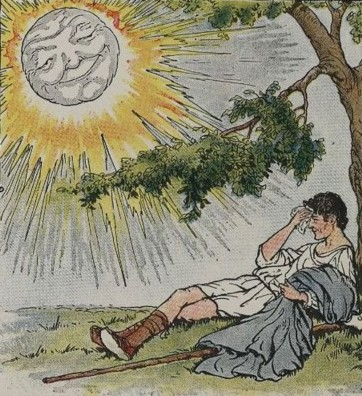
\includegraphics[scale=0.91]{sun.jpg}
% figure caption is below the figure
 \caption{Milo Winter illustration of Aesop Fable \textit{The North Wind and the Sun}, 1919; both natural forces wind and sun are anthropomorphized with a human face; picture source: wikipedia}
 \label{fig:1}       % Give a unique label
 \end{figure}
 

\subsection{Explanations for Anthropomorphism}
\label{sec:3.1}

	According to Lee \textit{et al.} \cite{lee_human_2005}, there are two main perspectives in explaining people's tendency to anthropomorphize. The first one explains anthropomorphism from the design of the artifact (anthropomorphic form in the design). It assumes that humans directly respond to life-like or social cues that an object or system emits, without thoughtful mental processing, by simply applying stereotypes and heuristics to it. In fact, from early childhood on, humans are inherently well-trained to perceive life \cite{epley_seeing_2007}. Schmitz \cite{schmitz_concepts_2011} describes that within the visual scope of design, the outer appearance can have an important impact on the overall perception of an object. The basic assumption here is that if an artifact appears much like a human it is likely to be treated similar to a human. If this explanation of anthropomorphism is correct, people may respond automatically to social cues emitted by a robot, and apply human-human social schemas and norms to these interactions.
	
	The second perspective applies a human-centered, cognitive viewpoint where anthropomorphism is described through people's specific mental model they construct about how an artifact works the way it does. According to v. Foerster \hl{ref} \textit{"we anthropomorphize because it allows us to explain things we do not understand in terms that we do understand, and what we understand best is ourselves as human beings"} \cite{hegel_understanding_2008}. This is consistent with the \hl{familiarity thesis (18)} \cite{hegel_understanding_2008} which claims we understand the world based upon a mental model of the world that we are most familiar with. Consequently, people tend to thoughtfully develop a mental model of agents in their environment and make inferences about it based on what is familiar to them. This point of view implicitly builds on a person's ability to attribute mental states to oneself and others, which is called \textit{Theory of Mind}. A theory of  mind for other agents enables us to attribute intentionality to those agents \cite{leslie_pretense_1987,admoni_multi-category_2012}. If a system behaves much like a human being (e.g. emits a human voice), people's mental model of the system's behavior may approach their mental model of humans, though the model may differ in some important aspects \hl{ref? Schmitz?}. In turn, people's estimation of a robot's `knowledge' and its capabilities / abilities affects the way they relate to it. Research examined the validity of the mental model concept with various kinds of robots \cite{schmitz_concepts_2011,kiesler_mental_2002}. Findings suggest that people tend to hold richer mental models about anthropomorphic robots in contrast to mechanic ones \cite{kiesler_mental_2002}.
  
\hl{here or later? : familiarity thesis does probably not hold after one get's acquantained with a robot.}

\subsection{Insights from Social and Developmental Psychology}
\label{sec:3.2}

	To understand the social phenomenon of anthropomorphism better, it makes sense to take a look at studies and explanations from (developmental) psychology. The phenomenon of attributing intentions and \hl{animacy} to simple shapes based on motion has been intensively studied in (developmental) psychology. Two famous studies on the perception of and attribution to simple things have been done in the mid 1940s: Heider and Simmel's work on the \textit{attribution theory} \cite{heider_experimental_1944} and Michotte's studies on \textit{the perception of causality} \cite{michotte_perception_1963}. In both experiments, participants viewed animations of simple shapes, such as circles or triangles (see Figure \ref{fig:2}). Asked to describe what they observed, interestingly, most people developed elaborate stories, attributing motivations, emotions and relationships between the objects.

\begin{figure}\centering
% Use the relevant command to insert your figure file.
% For example, with the graphicx package use
  
\includegraphics[scale=0.6]{heider-simmel_animation.jpeg}
% figure caption is below the figure
 \caption{Fritz Heider and Mary-Ann Simmel's animated film to study people's tendency to attribute animacy and intention to simple shapes; \textit{An experimental study of apparent behaviour}, 1944}
 \label{fig:2}       % Give a unique label
 \end{figure}

	What is a person's motivation to attribute human characteristics to simple geometric shapes, or more sophisticated, anthropomorphic shapes, animated or not? Irrespective of the artifact's characteristics, there are psychological theories to explain the phenomenon. An interesting recent psychological theory of anthropomorphism (also related to robotics) is provided by Epley, Waytz, and Cacioppo \cite{epley_seeing_2007}. The authors established a three-factor theory of when people are likely to anthropomorphize based on psychological determinants. Namely, the theory suggests that some people are more likely to anthropomorphize when:

\begin{itemize}
	\item anthropocentric knowledge is accessible and applicable to the artifact (\textit{elicited agent knowledge}),
	\item they are motivated to explain and understand the behavior of other agents (\textit{effectance motivation}), and
	\item they have the desire for social contact and affiliation (\textit{social motivation}).
\end{itemize}

	Epley \textit{et al.} describe that \textit{elicited agent knowledge} is a \textbf{cognitive determinant  of anthropomorphism} which is understood as the activation of knowledge about humans (or the self) when making inferences about non-human agents. One basic reasons for this are a person's physical constraints of being a human and nothing else. Consequently, one has no other experience than the self and in turn people tend to make inferences about others' mental states by relying inordinately on their own mental states. \footnote{Using one's own mental states and characteristics as a guide when reasoning about other humans is ego-centrism; when reasoning about non-human agents is anthropomorphism. See Epley, 2007 \textit{et al.} \cite{epley_seeing_2007}} Also empirical findings suggest that knowledge about humans in general, or self-knowledge in particular, is likely to serve as a readily accessible base for induction when reasoning about non-human agents. This tendency is usually stronger in young children and decreases with cognitive development and the learning to distinguish the self from other humans, and non-human agents. 
	
	Both \textit{effectance} and \textit{sociality} are \textbf{motivational determinants of anthropomorphism}. \textit{Effectance} is understood as the motivation to interact effectively in one's environment: understand, predict, \hl{reduce uncertainty (this feeds again our hypothesis that as soon as a robot is not uncertain anymore, there is no need to keep on anthropomorphizing it)} about one's environment and the agents that inhabit it. According to Epley \textit{et al.}, anthropomorphism serves as one way to reduce uncertainty and increase comprehension of events in one's environment. They mention for instance, children (as they are in their early stages of life) appear to be more likely to anthropomorphize than adults, as they might feel more uncertain within their environment.
	\textit{Sociality} describes the motivation for social contact, social connection, and social approval from other agents. Importantly for anthropomorphism, this social connection appears to be satisfied by connections with \hl{ \textit{"two of the most commonly anthropomorphized hon-human agents, namely pets and religious agents"}} \cite{epley_seeing_2007}. According to Epley \textit{et al.}, the motivation of being socially connected increases the tendency to anthropomorphize non-human agents because first sociality motivation increases the tendency to perceive human-like characteristics and traits even in non-human agents, and second it increases the tendency to search for sources of social connection in one's environment. Consequently, the authors suggest \textit{"[...] those who are chronically lonely should be more likely to anthropomorphize nonhuman agents than those who are more chronically connected"}. 
	
	\hl{BRIDGE}
	


\subsection{Anthropomorphism in Robotics}
\label{sec:3.3}
	
	Anthropomorphism is a commonly observed phenomenon in human-robot interaction. Studies showed that there are people who directly talk to their robot (even if it does not recognize speech), give it a name, greet it, wonder about its intentions or actions \cite{eyssel_anthropomorphic_2010,fink_anthropomorphic_2012,forlizzi_how_2007,fussell_how_2008,kiesler_anthropomorphic_2008}. It has frequently been described that people ascribe intentions or emotions to their domestic robot, such as to a Roomba vacuum-cleaning robot \cite{krumm_my_2007,sung_robots_2009} or their AIBO robotic dog \cite{friedman_hardware_2003}. However, people's tendency to anthropomorphize technologies has not only been observed with robots but described earlier in human-computer interaction and related to digital agents \cite{reeves_media_1996, nass_anthropocentrism_1995}. Though, the phenomenon seems to be more coined in human-robot interaction than in other human-machine interaction fields. What makes anthropomorphism special in robotics, is probably related to the (unique) characteristics of robots in contrast to other technologies. Robots are embodied, physical agents, autonomously acting right next to us, and able to respond intelligently to us and the environment. These are factors that seem to facilitate anthropomorphism, due to the nature of the phenomenon and its origins itself. In robotics, anthropomorphism is further encouraged through specific anthropomorphic design of a robot. But what is the interest, which underlies the efforts of enhancing anthropomorphism through specific anthropomorphic design in robots? Why does anthropomorphism seem to be so important in robotics? There is no one single answer to this question but certainly, developers and designers have discovered that anthropomorphism seems to be beneficial for human-robot relations, especially with socially interactive robots \cite{fong_survey_2003}. More concretely, it has been found that the appearance and function of a \hl{product (research in marketing?)}) impacts how people perceive it, interact with it, and build long-term relations with it \cite{bartneck_shaping_2004}. Consequently, the domain of (social) robotics tries to exploit this fact by enhancing anthropomorphism through anthropomorphic robots: \textit{"Applying anthropomorphism or zoomorphism changes the way how users try to understand and make sense of a [system] by projecting everyday \hl{expectations} of human and animalistic life onto it."} \cite{schmitz_concepts_2011}. Studies have further shown that perceived similarity between the user and the robot influences the intense of the participants' attributions towards the robot. Thus, anthropomorphism plays an important role in the design of robots as it is strongly related to the perception of intelligence, fun, the attribution of intentions and thus the predictability of the robot \hl{which ref??}.
	
	
	
%	Duffy defines anthropomorphism as "the tendency to attribute human characteristics to inanimate objects, animals and others with a view to helping rationalise their actions." \cite{duffy_anthropomorphism_2003}. This definition directly tries to give an explanation for why people tend to anthropomorphize robots, namely, in order to rationalize their actions, which seems to be effective as long as the robot is not very familiar to the human interaction partner. \hl{familiarity aspect LATER} Attributing familiar human-like qualities to a robot can serve to make the robot more familiar, explainable, or predictable \cite{epley_seeing_2007}. Further Duffy argues that anthropomorphism includes "attributing cognitive or emotional states to something based on observation." \cite{duffy_anthropomorphism_2003} \hl{BRIDGE, explain better} This is important for the acceptance of socially interactive robots \cite{fong_survey_2003} in daily life environments. As robots have to deal with people's acceptance to become useful devices and collaboration partners for humans, anthropomorphic robot design is amongst other reasons used to make people anthropomorphize (or socialize) the robot, treat it socially, act empathetical toward it. 

	


	

	"[...] the experiment demonstrates that human beings implicitly attribute human-like qualities, such as mental states, to nonhuman agents. This finding was evident on a neurophysiological level as well as behavioural level." \cite{hegel_understanding_2008}
	


	


%%%%%%%%%%%%%%%%%%%%%%%%%%%%%%%%%%%%%%%%%%%%%%%%%%%%%%%%%%%%%%%%%%%%%%%%%
%
%
%
%				HUMAN-LIKE DESIGN IN ROBOTS
%
%
%
%%%%%%%%%%%%%%%%%%%%%%%%%%%%%%%%%%%%%%%%%%%%%%%%%%%%%%%%%%%%%%%%%%%%%%%%%


\section{Human-like Design in Robots}
\label{sec:4}

	Anthropomorphic design means an imitation of human form (or natural form, in a broader understanding) \cite{disalvo_seduction_2003}. Concepts of anthropomorphic or other life-like forms can be found in a variety of interactive objects and effects of this design approach are studied in disciplines such as affective computing, tangible interaction or industrial design. In a robot, anthropomorphic design can be realized in \textit{1)} a robot's physical (visible) form / shape (embodiment / appearance), \textit{2)} its behavior (e.g. motion), and \textit{3)} the kind of interaction / communication (e.g. modality) that it enables or triggers. Especially socially interactive robots often make use of `human social' behavior cues, such as express / perceive emotions, communicate with high-level dialogue, learn / recognize models of other agents, establish / maintain social relationships, use natural cues (gaze, gestures, etc.), exhibit distinctive personality and character, or learn / develop social competencies \cite{fong_survey_2003}.
 

\subsection{Human-like embodiment (form / shape)}
\label{sec:4.1}

	The degree of human-like shape in a robot, also its morphological similarity, is the extent to which a non-human agent's observable features look human-like. \cite{epley_seeing_2007} Fong \textit{et al.} classify four categories of a robot's aesthetic form: \cite{fong_survey_2003}
	
\begin{itemize}
	\item anthropomorphic: structurally and functionally similar to a human
	\item zoomorphic: imitation of forms of living creatures, e.g. animal or pet design
	\item caricatured: using a character or caricature form, e.g. inspired from animation
	\item functional: reflecting the task a robot should perform
\end{itemize}

	For some robots, it seems to be difficult to assign them to only one of these categories. How to categorize, for instance, a mainly functional robot which has only a human-like head? It is also interesting that each of the four categories follows specific design principles to fulfill different goals. For instance, zoomorphic robots seem to help creating a "companionship" relation (e.g. similar to the owner-pet relation), whereas the anthropomorphic design seems to foster rather a human-social relation between the robot and the human and also tries to give the impression of the robot being a more sophisticated interaction partner \cite{disalvo_all_2002,fong_survey_2003,kiesler_mental_2002}. Accordingly, a robot's functionality should be reflected in it's design because it strongly impacts what kind of expectations people have of the robot \hl{ref, matching hypothesis}: \textit{"The device's visual appearance will often shape first impressions and can therefore play a considerable role in establishing first expectations."} \cite{schmitz_concepts_2011} What however is the best design for a multi-purpose robot that not only vacuums floors but also aims to interact socially with the user? This seems to be a fundamental question in HRI and the design of robots. Interestingly, it has been observed that body parts of a robot that are associated with senses could indicate that the robot is capable of perceiving the corresponding modality (e.g. eyes suggest seeing and ears hearing, respectively. \cite{schmitz_concepts_2011} Schmitz calls this notion \textbf{anthropomorphic affordances}, which describe affordances of an artifact that are impacted by its anthropomorphic shape and suggest to a user a  specific action or interaction. Consequently, if a more human-like shaped robot leads to higher expectations from the user side, it seems to be exeptionally difficult at this moment, to build a satisfying anthropomorphic robot. Moreover, there are also practical affordances that a robot's shape brings along. A legged robot is supposed to be able to walk and climb stairs whereas a wheeled one would probably not be able to do so. \hl{Sullivan: form follows funtion!}
	
\subsection{Human-like behavior}
\label{sec:4.2}

	Besides anthropomorphic shape, also a robot's behavior, e.g. the particular way of how it moves, can be human-inspired (which is in fact often defined by its morphology). According to Epley \textit{et al.} \textit{"at least two dimensions of similarity seem particularly important for anthropomorphism to occur -- similarity in motion and similarity in morphology"} \cite{epley_seeing_2007}. Similarity in motion might not only be walking on two feet but also the speed of movements of a robot, which when adapted to a human, have a positive effect on the usability and perception of the robot from the user cite \hl{ref!!}. The aspect is less important for robots in automation (e.g. assembly lines, production) which usually do not directly interact with humans.
	
	Another aspect of human-like behavior in robots is autonomy and pro-activity. Schmitz argues that both can be a fundamental strategy in order to evoke anthropomorphic / zoomorphic interpretation \cite{schmitz_concepts_2011} \hl{ref 33}. \hl{more on autonomy and pro-activity, transparency}

	"On a next level, \textbf{stereotypical behaviour}, which expresses e.g. shyness of curiosity, addresses more complex processes but adds essentially to anthropomorphic strategies [38] [46]." \cite{schmitz_concepts_2011}
	
	\hl{Severin: mention the need to be "complete enough not to be predictable" --> toys that are predictable are quickly boring and humans are really good at identifying simple logical behaviors. / Julia: role of uselessness in robots, surprise factor}


\subsection{Human-like interaction / communication}
\label{sec:4.3}


	"The mere \textbf{presence of voice} is another strong trigger for anthropomorphic perception \hl{(33)}, irrespective of contents and sounds." \cite{schmitz_concepts_2011}

	"Besides speech, the acoustic channel can be used to deliver alternative feedback that resembles \textbf{life-like, physiological sounds or haptics} instead of conventional feedback, for example pulse, breath, snore or cough [...]." \cite{schmitz_concepts_2011}


Others: proxemics


%%%%%%%%%%%%%%%%%%%%%%%%%%%%%%%%%%%%%%%%%%%%%%%%%%%%%%%%%%%%%%%%%%%%%%%%%
%
%
%
%				DOES ANTHROPOMORPHISM MAKE ROBOTS MORE SOCIAL?
%
%
%
%%%%%%%%%%%%%%%%%%%%%%%%%%%%%%%%%%%%%%%%%%%%%%%%%%%%%%%%%%%%%%%%%%%%%%%%%


\section{Does anthropomorphism make robots more social?}
\label{sec:5}

	In general, it is suggested that increasing human-likeness of a robot	 will lead to more perceived \textit{affinity} from the human side \cite{mori_uncanny_1970}. This theoretical concept is also supported by psychological determinants of perceiving human-likeness in something non-human: \textit{"the more similar in appearance, the more people are likely to use themselves as a source of induction and anthropomorphize these nonhuman agents"} \cite{epley_seeing_2007}. Further, empirical studies have shown that robots with human-like forms can enhance social responses from humans which in turn can have a positive impact on acceptance \cite{venkatesh_theoretical_2000,duffy_anthropomorphism_2003,goetz_cooperation_2002}.  People responded more positively to an artifact that displayed human-like behavioral characteristics (emotions, facial expression) in contrast to a purely functional design \cite{eyssel_anthropomorphic_2010,krach_can_2008,reeves_media_1996,riek_how_2009}. Overall, these results suggest that human-like features in robots enhance anthropomorphism, and in turn create a social view toward the robot.


	"The anthropomorphic design of human-machine interfaces is inevitable. The important criterion is to seek a balance between people's expectations and the machines capabilities." \cite{duffy_anthropomorphism_2002}

	"What is the ideal set of human features that could supplement and augment a robots  social functionality?" \cite{duffy_anthropomorphism_2002}


	Though, the 'anthropomorphic design principle" seems beneficial, it also raises ethical issues and has been reviewed critically in terms of acceptance. How far do we want a robot to resemble a human or act like a human?

	Findings that support anthropomorphic form in robots because they found people respond with anthropomorphizing these kind of robots, and in turn act more social toward them or accept them more easily:

	\hl{empathy --> check Iolanda's paper}

\subsection{Socially interactive robots}
\label{sec:5.1}

Evaluation and classification of social robots


\subsection{Too much human-likeness?}
\label{sec:5.2}

\begin{figure}\centering
% Use the relevant command to insert your figure file.
% For example, with the graphicx package use
  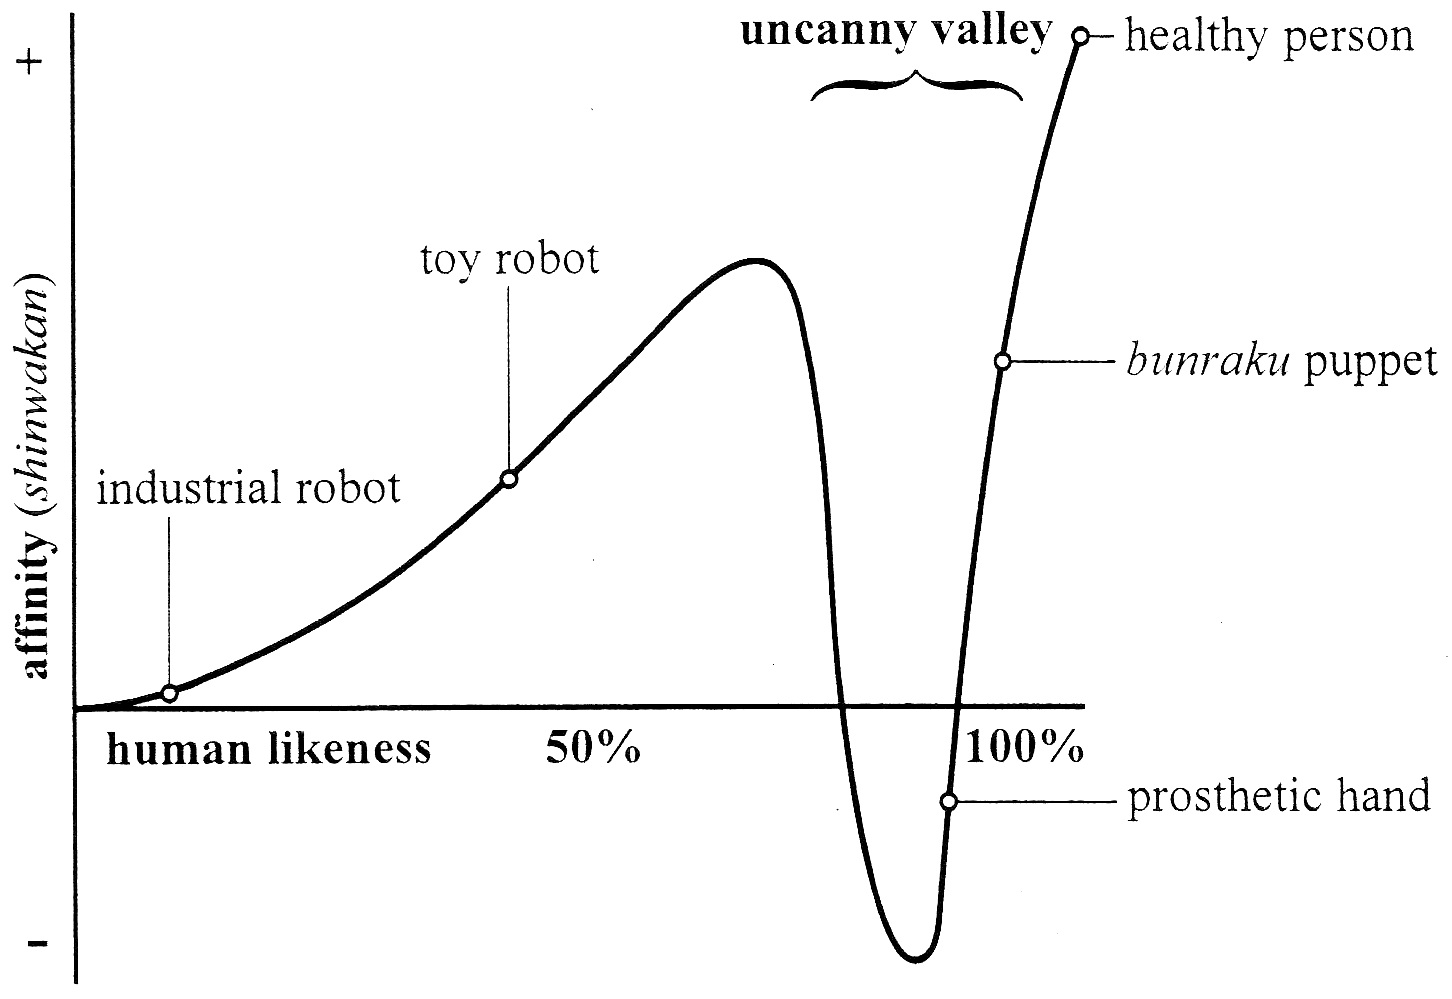
\includegraphics[scale=0.6]{uncanny-valley.jpg}
% figure caption is below the figure
 \caption{Mashiro Mori, illustration of the \textit{Uncanny Valley}, originally from 1970; picture from a manuscript version of \cite{mori_uncanny_2012}}
 \label{fig:2}       % Give a unique label
 \end{figure}




	The \textit{Uncanny Valley} hypothesis \cite{mori_uncanny_1970} models people's reactions to technologies that resemble a human too close while still not being one (see Figure). The theory hypothesizes that a person's response to a human-like robot would abruptly shift from empathy to revulsion as it approached, but failed to attain, a lifelike appearance \cite{mori_uncanny_1970}. Starting with low degrees of anthropomorphic cues in a robot, humans seem to readily accept and prefer them compared to purely mechanical robots. In general, one can say that up to a certain (yet not very well defined) degree, the more human-like the robot, the more affection it can engender through familiar communication references.
	
	when slowly increasing its human-likeness, the more affection 
	
The idea of the hypothesis follows Freud's description of the uncanny (a translation from the German word `unheimlich') \hl{ref Freud, The Uncanny}: "it derives its terror not from something externally alien or unknown but - on the contrary - from something strangely familiar which defeats our efforts to separate ourselves from it". \cite{hegel_understanding_2008}

	Also: Simulation Theory

	Findings that oppose anthropomorphic design in robots as people respond negatively to it:
	
	
%%%%%%%%%%%%%%%%%%%%%%%%%%%%%%%%%%%%%%%%%%%%%%%%%%%%%%%%%%%%%%%%%%%%%%%%%
%
%
%
%				SKEPTICAL REVIEW OF ANTHROPOMORPHISM IN HRI
%
%
%
%%%%%%%%%%%%%%%%%%%%%%%%%%%%%%%%%%%%%%%%%%%%%%%%%%%%%%%%%%%%%%%%%%%%%%%%%

\section{Does anthropomorphism make robots more social?}
\label{sec:6}

We believe that the prevalent mostly observed anthropomorphic stances in short-term experiments do not fully embrace this complex social phenomenon. For instance, when reading through literature on anthropomorphism in robotics one can get the impression that it is taken as a given fact that once people attribute human characteristics to a robot, they will always keep on doing so.
	
	short term
	
	lab context
	
	fake comparison of different robots that are not appropriate for comparison	
	
	
%%%%%%%%%%%%%%%%%%%%%%%%%%%%%%%%%%%%%%%%%%%%%%%%%%%%%%%%%%%%%%%%%%%%%%%%%
%
%
%
%				OUR MODEL
%
%
%
%%%%%%%%%%%%%%%%%%%%%%%%%%%%%%%%%%%%%%%%%%%%%%%%%%%%%%%%%%%%%%%%%%%%%%%%%

\section{Initial Model of the Dynamics of Anthropomorphism}
\label{sec:7}	


\begin{figure*}[htb]
\centering


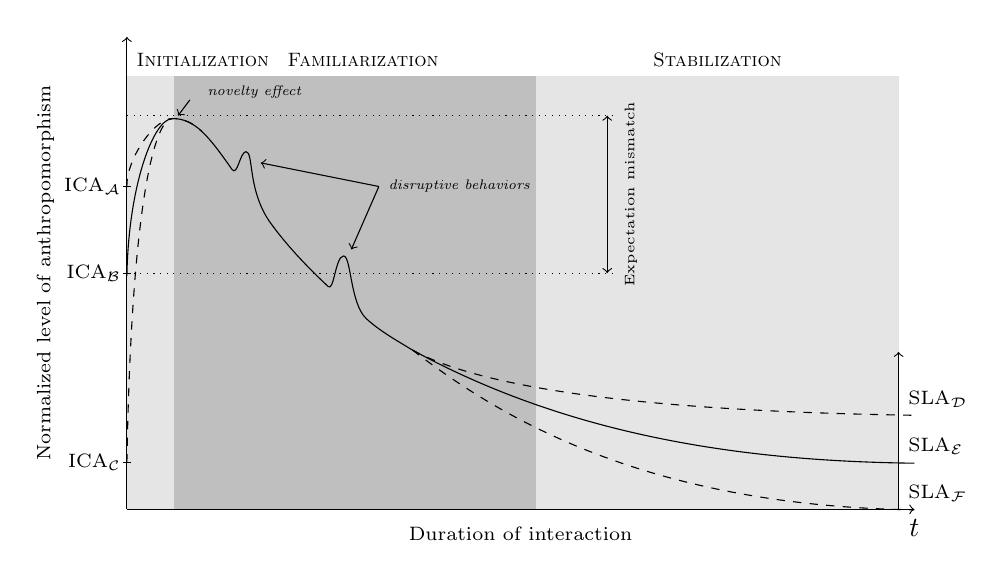
\begin{tikzpicture}

% background shading
\path[fill=gray!20] (0,0) rectangle (0.6,5.5);
\path[fill=gray!50] (0.6,0) rectangle (5.2,5.5);
\path[fill=gray!20] (5.2,0) rectangle (9.8,5.5);
\draw(0,5.5) node[anchor=south west] {\scriptsize \sc Initialization};
\draw(3,5.5) node[anchor=south] {\scriptsize \sc Familiarization};
\draw(7.5,5.5) node[anchor=south] {\scriptsize \sc Stabilization};
% horizontal axis
\draw[->] (0,0) -- (10,0) node[anchor=north] {$t$};
\draw(5,-0.1) node[anchor=north] {\scriptsize Duration of interaction};


% vertical axis
\draw[->] (0,0) -- (0,6) node[anchor=east] {};
\draw(-0.8,3) node[rotate=90,anchor=south] {\scriptsize Normalized level of anthropomorphism};

\draw (-0.05, 3) -- (0.05, 3) node[anchor=east] {\scriptsize $\text{ICA}_{\mathcal B}$};
\draw (-0.05, 4.1) -- (0.05, 4.1) node[anchor=east] {\scriptsize $\text{ICA}_{\mathcal A}$};
\draw (-0.05, 0.6) -- (0.05, 0.6) node[anchor=east] {\scriptsize $\text{ICA}_{\mathcal C}$};

% vertical axis - end
\draw[->] (9.8,0) -- (9.8,2) node[anchor=east] {};
\draw (9.8, 0.8) node[anchor=west] {\scriptsize SLA$_\mathcal{E}$};
\draw (9.8, 1.4) node[anchor=west] {\scriptsize SLA$_\mathcal{D}$};
\draw (9.8, .2) node[anchor=west] {\scriptsize SLA$_\mathcal{F}$};


\draw[<-] (0.65,5) -- (0.8,5.2) node[anchor=east] {};
\draw (0.9,5.3) node[anchor=west] {\tiny \it novelty effect};


\draw[dotted] (0, 5) -- (6.2,5);
\draw[dotted] (0, 3) -- (6.2,3);
\draw[<->] (6.1,3) -- (6.1,5) node[anchor=east] {};
\draw (6.2,4) node[rotate=90, anchor=north] {\tiny Expectation mismatch};

\draw[<-] (1.7,4.4) -- (3.2,4.1) node[anchor=east] {};
\draw[<-] (2.85,3.3) -- (3.2,4.1) node[anchor=east] {};
\draw (3.2,4.1) node[anchor=west] {\tiny \it disruptive behaviors};
%%%%%
%% CURVES
%%%%
\begin{scope}[yscale=-1,shift={(-0.125,-0.4)}]

% output of inkscape2tikz
\path[draw=black]
    (0.1250,-2.5620) .. controls (0.1451,-3.7193) and (0.4645,-4.5602) ..
    (0.7044,-4.5633) .. controls (0.8413,-4.5633) and (0.9599,-4.5104) ..
    (1.0794,-4.3971) .. controls (1.1989,-4.2841) and (1.3191,-4.1185) ..
    (1.4588,-3.9181) .. controls (1.5287,-3.8183) and (1.5610,-4.1413) ..
    (1.6381,-4.1420) .. controls (1.7378,-4.1420) and (1.6515,-3.6434) ..
    (1.9554,-3.2280) .. controls (2.1466,-2.9667) and (2.3889,-2.7023) ..
    (2.6819,-2.4292) .. controls (2.7551,-2.3607) and (2.7727,-2.8119) ..
    (2.8771,-2.8180) .. controls (2.9742,-2.8180) and (2.9594,-2.2108) ..
    (3.1665,-2.0209) .. controls (3.3340,-1.8673) and (3.5379,-1.7527) ..
    (3.7508,-1.6236) .. controls (5.8366,-0.4852) and (8.0977,-0.2106) ..
    (10.1250,-0.1860);
\path[draw=black, dashed]
    (0.1250,-3.6924) .. controls (0.1103,-4.0298) and (0.4645,-4.5602) .. 
    (0.7044,-4.5633)
    (3.7508,-1.6236) .. controls (4.9579,-0.9555) and (8.1358,-0.8261) .. 
    (10.1250,-0.7946);
\path[draw=black,dashed]
    (0.1250,-0.1953) .. controls (0.1804,-3.3871) and (0.4645,-4.5602) .. 
    (0.7044,-4.5633) .. controls (0.8413,-4.5633) and (0.9599,-4.5104) .. 
    (1.0794,-4.3971)
    (3.7508,-1.6236) .. controls (4.7654,-0.8505) and (6.5955,0.3538) .. 
    (10.1250,0.4062);

\end{scope}

\end{tikzpicture}

\caption{Dynamics of anthropomorphism. We distinguish three main phases:
\emph{initialization}, \emph{familiarization} and \emph{stabilization}. In the
pre-interaction phase, users build an \emph{initial capital of
anthropomorphism} (ICA). Once the interaction starts, the level of
anthropomorphism increases due to the \emph{novelty effect}, and then decreases
to reach a \emph{stabilized level of anthropomorphism} (SLA).
During the interaction, unpredicted behaviors of the robot (\emph{disruptive
behaviors}) locally increase the level of anthropomorphism.}
\label{fig|dynamics}
\end{figure*}


In this section we outline the essence of our initial model of the dynamics of anthropomorphism. This work is still in progress. The ideas we discuss are still incomplete, and their implications for the design of (social) robots and human-robot interaction are still quite speculative. Nonetheless, we believe that even our initial model, incomplete as it is, provides lessons for the understanding and study of anthropomorphism in robotics. However, we view this paper as only setting the stage for further research, realizing full well that it raises many more questions than it answers.

We propose to go beyond the traditional perception of anthropomorphism in robotics as a static feature.  We rather suggest to understand anthropomorphism in HRI as a dynamic, and context-dependent process, which is likely to change over time and with growing user experience with the robot (which we assume comes along with a familiarization and better understanding of the robot). This viewpoint considers the so called \textit{novelty effect} which has been observed during long-term studies with innovative technologies and robots. In the following, we present our understanding of the dynamics of anthropomorphism and try to model this process as a function of time and growing experience.
 

\subsection{The Initial Capital of Anthropomorphism}
\label{sec:7.1}

	Initially, there is a given potential that a robot will be anthropomorphized. Our proposed function of anthropomorphism starts with this what we call \textit{initial capital} of anthropomorphism (ICA) at time point = 0, which describes the first (imagined) contact to the robot. This time point can temporally be before the first real physical interaction with the robot, for instance, when a person learns about the existence of vacuum-cleaning robots (\textit{e.g.} when one sees an advertisement of the robot, or discusses about it with a friend). In this phase of "pre-interaction", people form initial expectations toward the robot and imagine how they will use / interact with it, before they actually start interacting with it in real. Therefore, the time point = 0 can be understood as user experience = 0. \hl{[pre-adoption, rogers]} How can we hypothetically quantify the ICA? We argue, that the potential to anthropomorphize a robot is mainly determined by three factors, which we would like to introduce as the "Three P's":  
	
\begin{enumerate}

	\item The \textbf{personality} of the human user: Psychological characteristics / determinants that influence a person's tendency to anthropomorphize artifacts, see \cite{epley_seeing_2007}.
	
	\item The human user's \textbf{perception} of the robot: Characteristics of the robot's form, behavior, and interaction modalities (anthropomorphic design), see \cite{fong_survey_2003}.
	
	\item The real or imagined \textbf{purpose} of the robot: The task context and role in which the robot is used / experienced (environmental context), see \cite{joosse_what_2013}.

\end{enumerate}	

	The ICA builds the sum of some hypothetical values for the "Three P's" and ranges between the theoretical values of 0 and 1.
	For \textbf{personality}, we suggest to apply Epley \textit{et al.}'s psychological \textit{"Three Factory Theory"} of anthropomorphism. For instance, children generally tend to anthropomorphize objects more than adults. Also, a person who lacks social connection is said to be more likely to anthropomorphize. Both aspects would increase the ICA.
	For \textbf{perception}, we understand that a robot that follows an anthropomorphic design (e.g. NAO) leads to a higher ICA than a rather functional robot (e.g. Roomba). Also, a robot that displays facial expressions would increase the ICA. However, \hl{as discussed before} a classification of the "amount" of anthropomorphic design in a robot, as for instance suggested by Fong \textit{et al.} \cite{fong_survey_2003}, can be difficult.
	For \textbf{purpose}, we propose that the real or imagined context in which a robot is used, impacts how far the robot will be attributed human-social characteristics. We	draw on findings such as presented in Joosse \textit{et al.}. The authors showed that when the same robot (NAO) is used in a different task context (cleaning task \textit{vs.} tour guide), this influences the perception of the "personality" of the robot. In general, we think that a robot which is (imagined to be) used in a social, entertaining or playful context leads to a higher ICA than a robot which is used for a serious task (security, rescue, etc.). This idea receives support from \hl{XX (Kiesler / Goetz?)} work that revealed that people prefer a serious robot for serious tasks and a less serious robot for more playful tasks \hl{REF}. Also, we suggest that the environmental context in which people experience and interact with the robot impacts the ICA. When several people who might be friends interact simultaneously with the robot this might lead to an increased ICA \hl{study: people are more emotional when watching TV in company than when watching TV on their own}.






%%%%%%%%%%%%%%%%%%%%%%%%%%%%%%%%%%%%%%%%%%%%%%%%%%%%%%%%%%%%%%%%%%%%%%%%%
%
%
%
%				DISCUSSION
%
%
%
%%%%%%%%%%%%%%%%%%%%%%%%%%%%%%%%%%%%%%%%%%%%%%%%%%%%%%%%%%%%%%%%%%%%%%%%%

\section{Discussion}
\label{sec:8}


\subsection{Effect of Context of Use and Purpose of the Robot}
\label{sec:8.1}
Frederic: role of uselessness


\begin{description}
	\item[\textbf{Hypothesis 1}] A person's tendency to anthropomorphize a robot is impacted by the context of use and purpose of the robot. A social context and purpose of the robot increases anthropomorphism. \textit{(context and purpose of the robot)}
\end{description}



\subsection{Effect of Time and Familiarization}
\label{sec:8.2}

	The \textit{context of use} is related to the purpose (and functionality) of the robot and influences the user interaction experience. With \textit{time}, we refer to long-term interaction with the robot, which is related to what has been described as 'novelty effect' but also accounts for the user getting used to the robot. Consequently, we propose that anthropomorphism is not static but likely to change, due to what we call \textit{dynamics}, in space and time.


	As outlined in section \hl{XX}, the tendency to anthropomorphize is motivated by a person's wish to make sense of an agent which might be difficult to understand (in its functionality or behavior, for instance). In turn, a user might ascribe intentions or emotions to the system because the systems output was unexpected for the user. Based on this explanation, we estimate that when the user has familiarized herself / himself with the system, thus reached the point of when the system is usable and explainable, the tendency to anthropomorphize decreases. Therefore, our second hypothesis is as follows: 

\begin{description}
	\item[\textbf{Hypothesis 2}] A person's tendency to anthropomorphize a robot decreases over time and with growing experience the person has with the robot. \textit{(familiarize oneself with the robot)}
\end{description}	
	

Given our first hypothesis from above, this might not hold over all contexts; more concretely, probably not in a social context of usage.


	Smart innovative devices, such as personal domestic robots, might demand from a human user spontaneous usage of an unfamiliar system. Such situations will require that a user should be able to build up a mental model quickly, which particularly holds for novice users \cite{schmitz_concepts_2011}.

	Eddy \textit{et aél.} points out that familiarity increases the tendency to anthropomorphize \cite{eddy_attribution_1993}.

	"As shown in several psychological experiments [13,24] and pointed out by Watt [25], familiarity may also ease social acceptance and even tend to increase people's tendency to anthropomorphize [16]." \cite{duffy_anthropomorphism_2003}

\subsection{Personal characteristic effects in anthropomorphizing}
\label{sec:8.3}



%%%%%%%%%%%%%%%%%%%%%%%%%%%%%%%%%%%%%%%%%%%%%%%%%%%%%%%%%%%%%%%%%%%%%%%%%
%
%
%
%				CONCLUSION
%
%
%
%%%%%%%%%%%%%%%%%%%%%%%%%%%%%%%%%%%%%%%%%%%%%%%%%%%%%%%%%%%%%%%%%%%%%%%%%


\section{Conclusion}
\label{sec:9}


	Anthropomorphism is a social phenomenon, which seems to be natural on one side and very complex on the other side. It is a mechanism within oneself that makes a human observer think and treat a non-human agent as if it would have some human (social) characteristics, and ascribe to it intentions, emotions, or thoughts, for instance. In accordance with other researchers, we also think that the term is sometimes misused or misunderstood \cite{duffy_anthropomorphism_2002}. Concerning robotics, we do not think that we can speak of anthropomorphism when a person simply refers to physical parts of a robot using terms that describe a human body, such as arm, head, fingers, etc.. We believe that this is not anthropomorphism in its true sense because the person might simply take advantage of the physically resembling shape instead of truly ascribing human (social) characteristics to the robot.




%\subsection{Subsection title}
%\label{sec:X.X}
%as required. Don't forget to give each section
%and subsection a unique label (see Sect.~\ref{sec:1}).
%\paragraph{Paragraph headings} Use paragraph headings as needed.
%\begin{equation}
%a^2+b^2=c^2
%\end{equation}

% For one-column wide figures use
% \begin{figure}
% Use the relevant command to insert your figure file.
% For example, with the graphicx package use
%  \includegraphics{example.jpg}
% figure caption is below the figure
% \caption{Please write your figure caption here}
% \label{fig:1}       % Give a unique label
% \end{figure}
%
% For two-column wide figures use
% \begin{figure*}
% Use the relevant command to insert your figure file.
% For example, with the graphicx package use
%  \includegraphics[width=0.75\textwidth]{example.eps}
% figure caption is below the figure
% \caption{Please write your figure caption here}
% \label{fig:2}       % Give a unique label
% \end{figure*}
%


\begin{acknowledgements}
AJung Moon, Aude Billard.\\
\end{acknowledgements}

% BibTeX users please use one of
 \bibliographystyle{spbasic}      % basic style, author-year citations
%\bibliographystyle{elsart-harv}
%\bibliographystyle{spmpsci}      % mathematics and physical sciences
%\bibliographystyle{spphys}       % APS-like style for physics
\bibliography{anthropomorphism}   % name your BibTeX data base


%\begin{thebibliography}{42}
%\providecommand{\natexlab}[1]{#1}
%\providecommand{\url}[1]{{#1}}
%\providecommand{\urlprefix}{URL }
%\expandafter\ifx\csname urlstyle\endcsname\relax
%  \providecommand{\doi}[1]{DOI~\discretionary{}{}{}#1}\else
%  \providecommand{\doi}{DOI~\discretionary{}{}{}\begingroup
%  \urlstyle{rm}\Url}\fi
%\providecommand{\eprint}[2][]{\url{#2}}
%
%
%\bibitem[{Young et~al(2008)Young, Hawkins, Sharlin, and
%  Igarashi}]{young_toward_2008}
%Young JE, Hawkins R, Sharlin E, Igarashi T (2008) Toward acceptable domestic
%  robots: Applying insights from social psychology. International Journal of
%  Social Robotics 1(1):95--108
%
%
%\end{thebibliography}

% Non-BibTeX users please use
% \begin{thebibliography}{}
%
% and use \bibitem to create references. Consult the Instructions
% for authors for reference list style.
%
% \bibitem{RefJ}
% Format for Journal Reference
% Author, Article title, Journal, Volume, page numbers (year)
% Format for books
% \bibitem{RefB}
% Author, Book title, page numbers. Publisher, place (year)
% etc
% \end{thebibliography}

%\paragraph{ }
%\begin{description}
$\newline$

\textbf{Julia Fink} is a PhD student in Human-Robot Interaction at EPFL. Her work focusses on the analysis of interaction, user experience and acceptance of robots in domestic spaces. She has a multi-disciplinary background in Media, Technology, Communication, and Interaction Studies. \\

\textbf{Dr. S\'{e}verin Lemaignan} is a postdoctoral researcher at EPFL. ...  \\

\textbf{Prof. Pierre Dillenbourg} is professor of learning technologies at EPFL. Former teacher in elementary school, he graduated in educational science (University of Mons, Belgium). He obtained a PhD in computer science from the University of Lancaster (UK), in the field of educational applications of artificial intelligence.  His work covers various domains of computer-supported collaborative learning (CSCL), ranging from novel interfaces for face-to-face collaboration (interactive furniture, tangibles, paper computing) to more cognitive projects on dual eye tracking.
%\end{description}


\end{document}
% end of file template.tex

